
\section{Problems with NHST}
\epigraph{The almost universal reliance on merely refuting the null hypothesis is a terrible
mistake, is basically unsound, poor scientific strategy, and one of the worst things that
ever happened in the history of psychology.}{Meehl, 1978}

Misconceptions about statistical significance
\begin{enumerate}
	\item A significant result means that the effect is important. 
	\begin{itemize}
		\item statistical significance is not the same thing as importance as p value is affected by sample size. small unimportant effects can also be statistically significant, if sufficiently large data is collected.
   	\end{itemize}
	\item A non significant result means that the null hypothesis is true
	\begin{itemize}
		\item Non significant result only tell use that the effect is not big enough to be found (given our sample size). Does not mean effect size is 0. As a sufficiently large sample size can make an infinitesimal effect size significant. so non significant result canot be interpreted as no difference between means or no relationship between variables.
	\end{itemize}
	\item A significant result means null hypothesis is false.
		\begin{itemize}
		\item NHST is the result of trying to find a system that can test which of
two competing hypotheses (the null or the alternative) is likely to be correct, it fails because
the significance of the test provides no evidence about either hypothesis. It only shows which hypothesis is likely to be correct
	\end{itemize}
\end{enumerate}

\section{All or Nothing thinking}
Using the p value of .05 encourages the \textbf{all or nothing} thinking: if p$<$.05, then it is significant, if p $>$ .05, then not significant.

However, this is ridiculous as sometimes, p value differ only very little yet people treat them as complete opposites (e.g. p = .0499 vs p = .0501, p value differ only by .0002)

e.g. if you do 10 studies, only 4/10 of the studies produce statistically significant result. All or nothing thinking will make you will say that the study is inconclusive. However if you look at the studies confidence intervals, even if some studies did not produce statistically significant result, they all are consistently positive. By looking at confidence intervals, we can have good reason that the effect may be greater than zero.

\begin{figure}[h]
	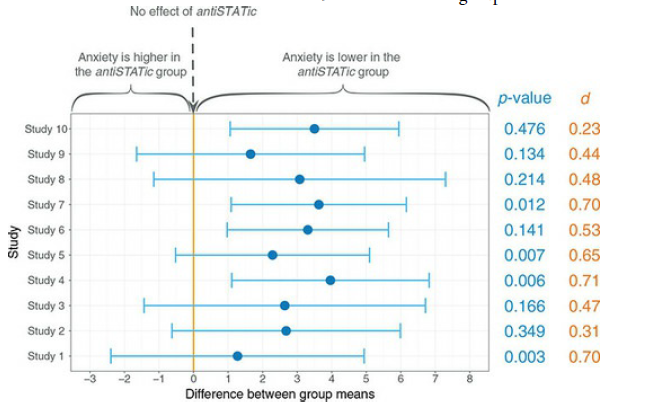
\includegraphics{Chapter 3 Pheonix of Statistics/confidenceinterval.PNG}
	\caption{4/10 are not statistically significant, but all the studies have positive difference between group means}
\end{figure}

\section{NHST is influenced by the intentions of the scientists}

NHST works on the principle that you make a Type I error in 5\% in an infinite number of repeated identical experiments (long run probability).
Both Type I and Type 2 errors are long run probability. It does not apply to individual studies. in an individual study, the probability is not .05 for alpha, it is either you have a Type I error (p = 1) or you don't (p=0).

\begin{center}
$p$-value is the probability of getting a test statistics at least as large as the one observed relative to all possible values of $t_{\text{null}}$ \emph{from an infinite number of identical replications of the experiments}
\end{center}

$p$-value is the frequency of the observed test statistics relative to all possible values that could be observed in the collective of identical experiments, \emph{with the exact same sampling procedure}.

E.g. You aim to collect 100 participants data, but only can find 93 participants. If you change your decision rule of computing p value based on 100 people to based on 93 people, result will change. i.e. if you compute p value based on df of 99 instead of df of 92, it is wrong. As you end up computing the relative frequency of the test statistics compared to all possible $t_{\text{null}}$s from experiments of size 93, but what you set out to do is to compare test statistic to all possible $t_{\text{null}}$s from experiments of size 100.
So the space of possible $t_{\text{null}}$s has been influenced by an arbitrary variable of \emph{availability of participants} rather than sticking to original scheme. 
The proper p-value you need to compute should be based on relative frequency of the observed test statistic compared to all possible $t_{\text{null}}$s from the collective of experiments where the intention was to collect 100 participants but (for the same reasons as in your experiment) only 93 participants were available. However, this p-value is too idiosyncratic to compute.

\section{Incentive Structures and Publication Bias}
Articles that have a significant finding are 7 times more likely to be published than non-significant ones. This is known as \textbf{publicatoin bias}, this bias is driven by reviewers rejecting non-significant result, and scientists not submitting articles with non significant results. 

"Publish or Perish" mentality and also incentive structures in Science only award individuals who have successful studies. and "success" is largely defined by a study being signiificant

\section{Researchers degrees of freedom}
\textbf{Researcher degrees of freedom} refers to the fact that a scientist has many decisions to make when designing and analysis a study. e.g. alpha, power, sample size, which statistical model to fit, how to deal with extreme scores, what variables to consider, what measures to use.

Researchers degrees of freedom can be misused to exclude cases to make the result significant.

NHST nurtures these temptations by fostering black and white thinking, in which significant results garner much greater personal rewards than non-significant ones. 

\section{p-hacking and HARKing}
\textbf{p-hacking} refers to researcher degrees of freedoms that lead to the selective reporting of significant p-values.

ways to p-hack:
\begin{enumerate}
\item deciding to stop collecting data at a point other than when the predetermined (prior to data collection) sample size is reached
\item including (or not) data based on the effect they have on the p-value.
\item including (or excluding) variables in an analysis based on how those variables affect the p-value
\item measuring multiple outcomes or predictor variables but reporting only those for which the effects are significant
\item merging groups of variables or scores to yield significant results, and transforming or otherwise manipulating, scores to yield significant p-values
\end{enumerate}

\textbf{HARKing} refers to the practice in research articles of presenting a hypothesis that was made after data collection as though it were made before data collection.

In both cases of p-hacking and HARKing, you are not controlling the Type I error rate as you are deviating from the process that ensures that it is control, so Type 1 errors will definitely be more than 5\%

\section{Effect Sizes}
Significance does not tell us about the importance of an effect. The solution to this criticism is to measure the size of the effect in a standardized way. 

\textbf{Effect size} is an objective and standardized measure of the magnitude of observed effect. 
standardized means that we can compare effect sizes across different studies that have measured different variables, or have used different scales of measurement. 

Most common effect sizes are: 1) Cohen's d, 2) Pearson's r, 3) odds ratio

\subsection{Odds ratio}

The odds of an event occuring are defined as the probability of an event occuring divided by the probability of an event not occuring.

$\text{odds} = \frac{\text{P(event}}{\text{P(no event)}}$ \\

\begin{table}[h]
	\begin{center}
	\setlength\tabcolsep{1cm}
	\begin{tabular}{|c|c|c|c|}
		\hline
		& Yes & No & Total \\
		\hline
		Singing & 12 & 88 & 100\\
		Conversation & 26 & 74 & 100\\
		\textbf{Total} & \textbf{38} & \textbf{162} & \textbf{200}\\
		\hline
	\end{tabular}
	\caption{data about effects of singing on saying yes to dates}
	\end{center}
\end{table}

e.g. We collected a data to undersrtand how much likely a person will say "yes" to a singer than to someone who starts a conversation.\\

\begin{equation*} % asterisk means no numbering
\begin{split}
\text{odds}_{\text{yes to a singer}} & = \frac{\text{Number of yes responses to a singer}}{\text{number of no responses to a singer}} \\ 
&= \frac{12}{88} = 0.14
\end{split}
\end{equation*}

\begin{equation*}
\begin{split}
\text{odds}_{\text{yes to a talker}} & = \frac{\text{Number of yes responses to a talker}}{\text{number of no responses to a talker}} \\ 
&= \frac{26}{74} = 0.35
\end{split}
\end{equation*}

\begin{equation}
\nonumber
\begin{split}
\text{odds}_{\text{ratio}} & = \frac{\text{odds}_{\text{yes to a singer}}}{\text{odds}_{\text{yes to a talker}}} \\ 
&= \frac{.14}{.35} = .4
\end{split}
\end{equation}

\section{Effect sizes compared to NHST}
\begin{itemize}
\item Encourage interpreting effects on a continuum and not applying a categorical decision rule such as "significant" or "not significant". 
\item While effect sizes are affected by sample sizes (larger sample yield better estimates of population size effect size), but unlike p-value, there is no decision rule attached to effect sizes, so the interpretation of effect sizes is not confounded by sample size (although it is important in contextualising the degree to which an effect size might affect the populaiton). i.e. effect sizes are less affected than p-values by things like early or late termination of data collection, or sampling over a time period, rather than until a set sample size is reached. 
\item While researcher degree of freedom still exists in that researchers could maximize effect sizes, but there is less incentives to do so as effect sizes are not tied to a decision in which effects of either side of a certain threshold have qualitatively opposite interpretations.
\end{itemize}